% ------------------------------------------------------------------------------
% TYPO3 CMS 8.1 - What's New (English Version)
%
% @author	Patrick Lobacher <patrick@lobacher.de> and Michael Schams <schams.net>
% @license	Creative Commons BY-NC-SA 3.0
% @link		http://typo3.org/download/release-notes/whats-new/
% @language	English
% ------------------------------------------------------------------------------
% LTXE-CHAPTER-UID:		dcfe6009-2200ad81-816c2edb-1f54c687
% LTXE-CHAPTER-NAME:	Backend User Interface
% ------------------------------------------------------------------------------

\section{Interfaz de Usuario de Backend}
\begin{frame}[fragile]
	\frametitle{Interfaz de Usuario de Backend}

	\begin{center}\huge{Capítulo 1:}\end{center}
	\begin{center}\huge{\color{typo3darkgrey}\textbf{Interfaz de Usuario de Backend}}\end{center}

\end{frame}

% ------------------------------------------------------------------------------
% LTXE-SLIDE-START
% LTXE-SLIDE-UID:		d0f905bc-9225e0d0-def65f30-238cf86e
% LTXE-SLIDE-ORIGIN:	5d3d70fa-92a2935e-f1cbdc1e-285ec842 English
% LTXE-SLIDE-TITLE:		Feature: #75497 - inline backend layout wizard
% LTXE-SLIDE-REFERENCE:	!Feature-75497-InlineBackendLayoutWizard.rst
% ------------------------------------------------------------------------------
\begin{frame}[fragile]
	\frametitle{Interfaz de Usuario de Backend}
	\framesubtitle{Asistente de Backend Layout Inline}

	Un nuevo tipo de renderizado ha sido añadido para renderizar el asistente del backend layout inline en FormEngine
	(en TCA: \texttt{'renderType' => 'belayoutwizard'}).

	\begin{figure}
		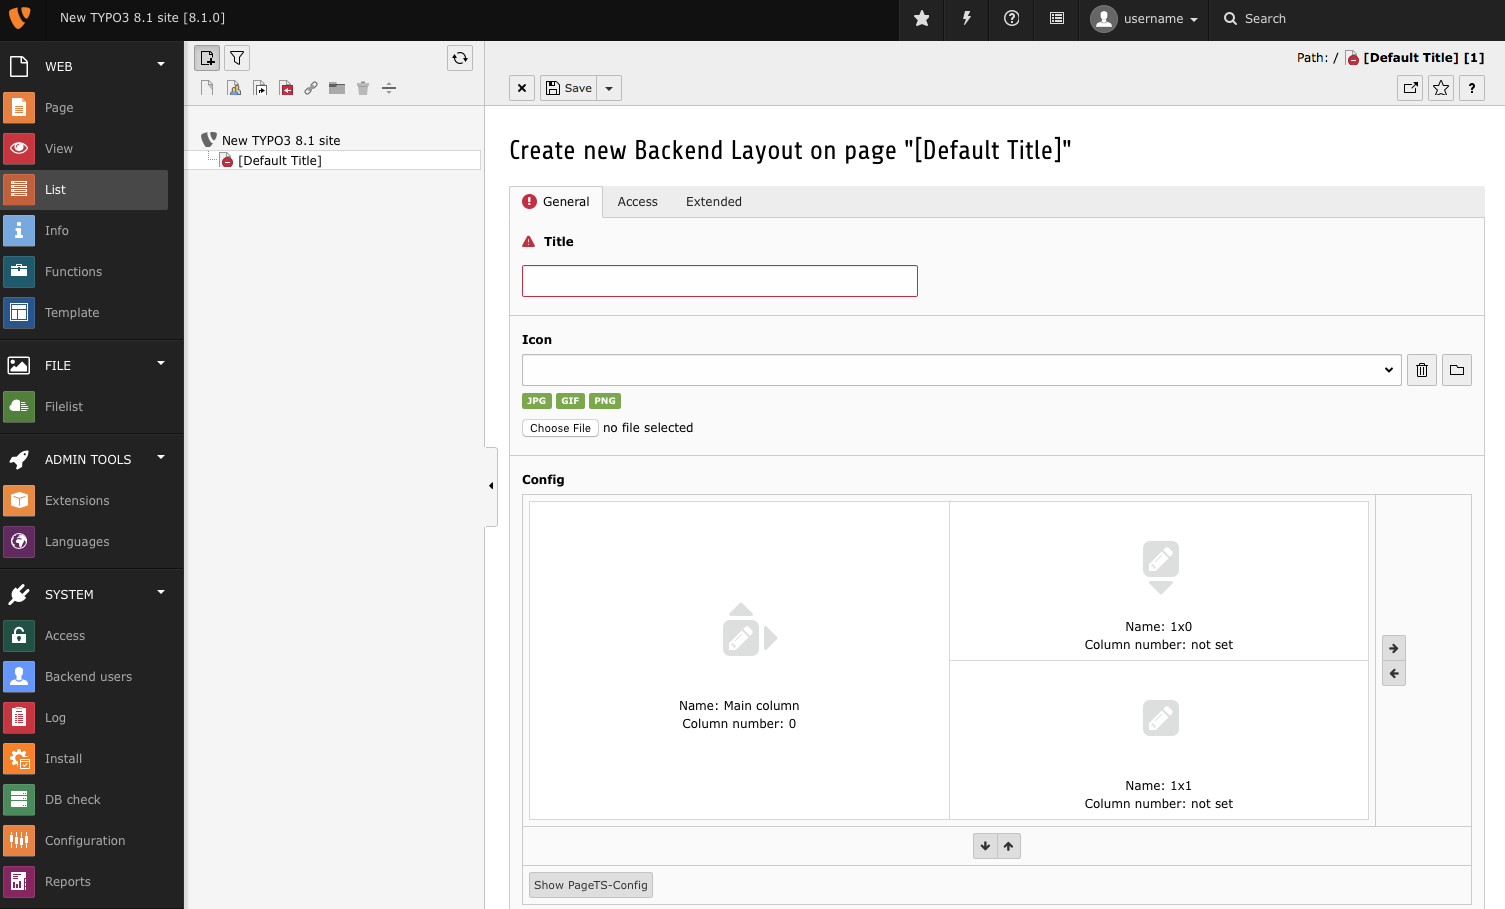
\includegraphics[width=0.70\linewidth]{BackendUserInterface/75497.png}
	\end{figure}

\end{frame}


% ------------------------------------------------------------------------------
% LTXE-SLIDE-START
% LTXE-SLIDE-UID:		741720cb-79240cd6-e3ca24f7-4e1b9557
% LTXE-SLIDE-ORIGIN:	7cab4dc0-cdfe9472-a3f0a874-dddf137d English
% LTXE-SLIDE-TITLE:		Feature: #75581 - Simplify cache clearing
% LTXE-SLIDE-REFERENCE:	!Feature-75581-SimplifyCacheClearing.rst
% ------------------------------------------------------------------------------
\begin{frame}[fragile]
	\frametitle{Interfaz de Usuario de Backend}
	\framesubtitle{Simplificar limpieza de Caché}

	El sistema de limpieza de caché ha sido simplificado eliminando opciones en el menú de limpiar caché y
	en la Herramienta de Instalación.

	\begin{itemize}

		\item \textbf{Vaciar cachés de frontend:}\newline
			\small
				Limpia las cachés de frontend y relacionadas con la página, como antes.
			\normalsize

		\item \textbf{Vaciar todas las cachés:}\newline
			\small
				Limpia las cachés relacionadas con el sistema, incluyendo el cargado de clases, localización,
				cachés de fichero de configuración de extensión y cachés opcode. Reconstruir esta caché
				puede llevar algo de tiempo.
			\normalsize

	\end{itemize}

	\begin{figure}
		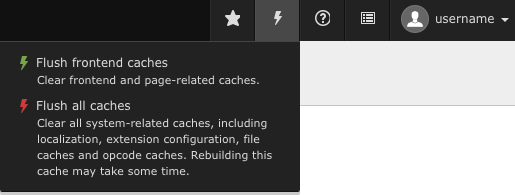
\includegraphics[width=0.45\linewidth]{BackendUserInterface/75581.png}
	\end{figure}

\end{frame}

% ------------------------------------------------------------------------------
% LTXE-SLIDE-START
% LTXE-SLIDE-UID:		e731797e-b9510ebc-3b4bb9ba-9c965058
% LTXE-SLIDE-ORIGIN:	e24e593c-fe9bcff9-c386db3a-79491de1 English
% LTXE-SLIDE-TITLE:		Rework Workspaces (1)
% LTXE-SLIDE-REFERENCE:	Rework Workspaces
% ------------------------------------------------------------------------------
\begin{frame}[fragile]
	\frametitle{Interfaz de Usuario de Backend}
	\framesubtitle{Workspaces Retrabajados (1)}

	\begin{itemize}

		\item El módulo workspace para manejar contenido de un stage ha sido reescrito y
			se integra mucho mejor en la apariencia visual del backend ahora

		\item Los editores se darán cuenta de inmediato, que encaja con la apariencia general
			debido a su base técnica con Twitter Bootstrap y jQuery

		\item Este cambio trae también un aumento de rendimiento y es un gran salto hacia delante
			para un backend TYPO3 más limpio y veloz con menos JavaScript

	\end{itemize}

\end{frame}

% ------------------------------------------------------------------------------
% LTXE-SLIDE-START
% LTXE-SLIDE-UID:		694eb575-09dbf8bf-a8036616-ae3757bb
% LTXE-SLIDE-ORIGIN:	fe9bcff9-e24e593c-79491de1-c386db3a English
% LTXE-SLIDE-TITLE:		Rework Workspaces (2)
% LTXE-SLIDE-REFERENCE:	Rework Workspaces
% ------------------------------------------------------------------------------
\begin{frame}[fragile]
	\frametitle{Interfaz de Usuario de Backend}
	\framesubtitle{Workspaces Retrabajados (2)}

	Capturas de pantalla del módulo workspace:

	\begin{figure}
		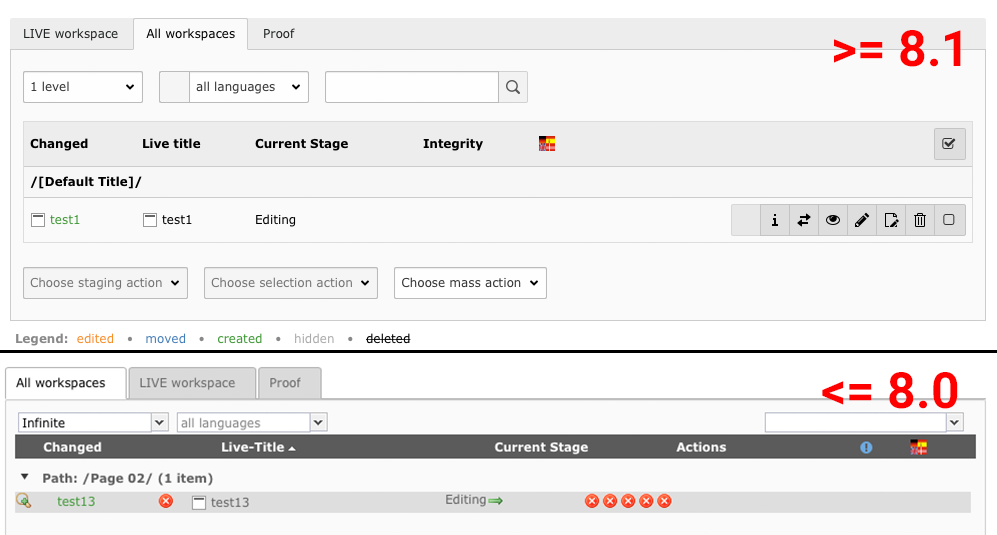
\includegraphics[width=0.85\linewidth]{BackendUserInterface/workspaces.png}
	\end{figure}

\end{frame}

% ------------------------------------------------------------------------------
